\documentclass[a4paper,12pt]{article}
\usepackage[T1]{fontenc}
\usepackage{imakeidx}
\usepackage{graphicx}
%\makeindex[columns=3, title=Alphabetical Index, intoc]

\begin{document}

\textbf{ISO}


\tableofcontents
\clearpage

 
\section{Introduction}
The International Organization for Standardization is an international standard-setting body composed of representatives from various national standards organizations.

The organization develops and publishes worldwide technical, industrial and commercial standards

\section{TCP-IP vs ISO}

ISO holds lots of standards and when it comes to network it classifies 7 layers whereas TCP/IP (for practical reasons) has only 4 because 3 layers of the standard ISO are actually representing the same physical reality

Here goes a quick example.

It's called ISO/OSI and stands for Open Systems Interconnection Protocolo and it's regulated by the International Organization of Standardization 
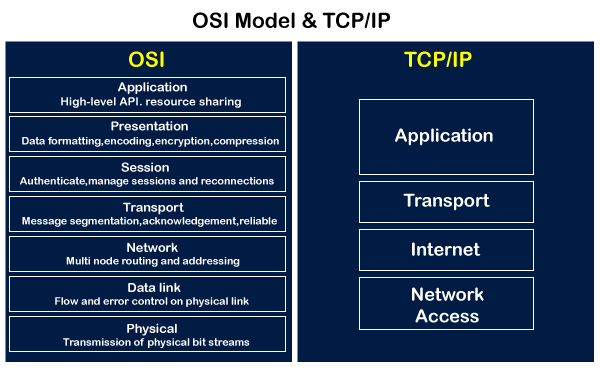
\includegraphics[width=15cm]{./osi-vs-tcp-ip2.png}

\section{ISMS 27001}

ISO/IEC 27001 is widely known, providing requirements for an information security management system (ISMS).
It enables organizations manage the security of \emph{assets} such as financial information, intellectual property, employee details or information entrusted by third parties

\section{Environmental 14001}
ISO 14001 sets the standard for Environmental Management Systems.

If you want to reduce waste management costs and demonstrate your commitment to protecting the environment, you need ISO 14001 certification. Implementing this global standard will also help you building trust with customers.

\section{Quality 9001}
ISO 9001 is used by businesses to continually monitor, manage and improve the quality of their products and services.

It is a powerful business improvement tool, providing the framework and guidance you need to help you consistently meet your customer’s expectations and regulatory requirements.

\clearpage

\printindex

\end{document}
